\chapter{Dãy số Đặc biệt}\label{ch:6}

Một vài dãy số xuất hiện thường xuyên trong toán mà chúng ta có thể nhận biết ngay được và đặt tên cho chúng. 
Có thể nói đến những ví thân thuộc như dãy $\langle 1,4,9,16,\ldots \rangle$.

\noindent

Trong Chapter 1,chúng ta đã tìm hiểu "số tam giác" 
$\langle 1,3,6,10,\ldots \rangle$,
trong Chapter 4 là dãy số nguyên tố
$\langle 2,3,5,7,\ldots \rangle$ 
còn Chapter 5 là dãy Catalan:
$\langle 1,2,5,14,\ldots \rangle$.

\noindent

Trong chương này, chúng ta sẽ làm quen với một vài những dãy số quan trọng nữa: 
dãy Stirling $n \brace k$ hoặc $\begin{bmatrix} n \\ k \end{bmatrix}$, 
dãy Euler ${\displaystyle \textstyle \left\langle {n \atop k}\right\rangle }$; 
những số trong các dãy này đều có liên quan phần nào đến hệ thức nhị phân 
$({n \atop k})$.
Cuối cùng sẽ là những dãy như Harmonic series, Bernoulli series và Fibonacci.

\section{Dãy Stirling}

\noindent 

Chúng ta bắt đầu với dãy thân thuộc với hệ thức nhị phân,dãy Stirling.
Dãy này có 2 loại, thường được gọi đơn giản là "Dãy Stirling dạng 1 và dạng 2". 
Mặc dù bản thân dãy số có đóng góp quan trọng vào lịch sử và những ứng dụng đa dạng,
chúng vẫn chưa có một ký hiệu chính thức. Thông thường, chúng ta ký hiệu 
$\begin{bmatrix} n \\ k \end{bmatrix}$  
cho số Stirling loại 1 và
${\displaystyle \textstyle \left \{ {n \atop k} \right \} }$
cho số Stirling loại 2 (theo cách ký hiệu của Jovan Karamata).

\noindent 

Bảng 258 và 259 biểu diễn các giá trị của
$\begin{bmatrix} n \\ k \end{bmatrix}$  
và 
${\displaystyle \textstyle \left \{ {n \atop k} \right \} }$, 
với $(n,k) \leq 9$. Khi nói đễn dãy "1,7,6,1" thì có thể đó là 
$\begin{bmatrix} n \\ k \end{bmatrix}$
và dãy "6,11,6,1" thì là 
${\displaystyle \textstyle \left \{ {n \atop k} \right \} }$, 
cũng giống như cách mà chúng ta cho rằng dãy "1,4,6,4,1" là $({n \atop k})$ khi $n = 4$

% Insert bảng 258 và bảng 259 vào đây

\subsection{Stirling loại 2}


Dãy Stirling loại thứ 2 thường xuất hiện nhiều hơn cả,nên chúng ta hãy nói về nó trước. 
Chúng ta có thể định nghĩa 
${\displaystyle \textstyle \left \{ {n \atop k} \right \} }$
là cách chia $n$ số vào $k$ subset không rỗng. 
Ví dụ,ta có 7 cách chia một dãy 4 phần tử vào 2 phần: 

\marginpar{(Stirling đã xét loại thứ 2 trước trong sách của ông. \cite{citation343})}

\begin{equation} 
    \begin{aligned}
        \left\{ 1,2,3 \right\} \cup \left\{ 4\right\} \\
        \left\{1,2,4\right\} \cup \left\{ 3\right\} \\
        \left\{ 1,3,4 \right\} \cup \left\{ 2\right\} \\
        \left\{2,3,4 \right\} \cup \left\{1 \right\} \\
        \left\{1,2\right\} \cup \left\{ 3,4\right\} \\
        \left\{ 1,3\right\} \cup \left\{ 2, 4\right\} \\
        \left\{1,4\right\} \cup \left\{2,3\right\} \\ 
    \end{aligned} \label{eq:6.1}
\end{equation}

\indent
Vậy nên $\displaystyle \textstyle \left \{ {4 \atop 2} \right \} = 7$.
Một điều thú vị đó là, những ngoặc $\{$ và $\}$ dùng để định nghĩa set 
được dùng để định nghĩa số Stirling trong trường hợp này.
Cách ký hiệu này giúp ta có thể hiểu 
$\left \{ {n \atop k} \right \}$ 
như "n subset k".

\indent
Ta xét một số trường hợp của $k$:

\begin{itemize}
    \item Nếu $(k,n) = (1,0)$: Có $0$ cách chọn $0$ phần tử vào $1$ subset. 
    \item Nếu $k = 1,n > 0$: 
            \\Chỉ có $1$ cách chọn $n$ phần tử vào $1$ subset,chính là dãy ban đầu.
    \item Nếu $k = 2$: \\
        Có thể dễ dàng thấy rằng, $n = 0$ thì sẽ có $0$ cách chia. 

        Xét dãy $n,(n > 0)$ phần tử và 2 subset sẽ được chia,ta có thể thấy 
        một trong 2 set sẽ chứa phần tử cuối và một vài phần tử của $n - 1$ phần tử 
        còn lại. Tổng cộng sẽ có $2^{n - 1}$ cách chia các phần tử đấy vào 2 subset 
        và trừ đi trường hợp một trong 2 subset là rỗng, vậy ta có kết quả là:
        \begin{equation}
            \begin{aligned}
                \left \{ {n \atop 2} \right \} = 2^{n - 1} - 1 \\
                n \in \mathbb{Z^+}
            \end{aligned} \label{eq:6.2}
        \end{equation}
\end{itemize}

\indent
Chúng ta có thể sử dụng cách lập luận vừa xong để suy được công thức truy hồi tính 
$\left \{ {n \atop k} \right \}$ với mọi k:
    \begin{itemize}
        \item Nếu ta đặt phần tử cuối cùng thành một nhóm riêng. \\
            Lúc đó ta sẽ còn $k - 1$ nhóm và $n - 1$ phần tử và
            $\left \{ {n - 1 \atop k - 1} \right \}$ cách chọn cho phần còn lại.
        \item Nếu ta cho phần tử cuối cùng vào $k$ nhóm hiện có.
            Sau khi bỏ phần tử cuối cùng đi,ta còn $n - 1$ phần tử và $k$ nhóm để 
            phân chia, $\left \{ {n - 1 \atop k} \right \}$ cách. Vì ta đẩy phần tử 
            cuối cùng vào một trong $k$ nhóm nên cũng có $k$ cách 
            chia $n - 1$ phần tử còn lại. Vậy tổng số sẽ là 
            $k \cdot \left \{ {n - 1 \atop k} \right \}$ cách
    \end{itemize}
Vậy
\begin{equation}
    \begin{aligned}
        \left \{ {n \atop k} \right \} = 
        k \cdot \left \{ {n - 1 \atop k} \right \} + 
        \left \{ {n -1 \atop k - 1} \right \} \
        \forall \  n \in \mathbb{Z^+}
    \end{aligned} \label{eq:6.3}
\end{equation}

\subsection{Stirling loại 1}
Sự khác nhau giữa định nghĩa của loại 1 và loại 2 đó chính là
ở loại 2 chúng ta chia các phần tử vào những cycles (cách sắp xếp vòng tròn ?). 

Cycle có thể hiểu như là một cách sắp xếp vòng tròn như hình sau:

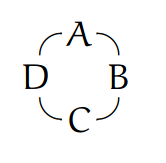
\includegraphics[width=0.25\textwidth]{assets/chapter6/cycle.png}

Cycle trong hình có thể được viết gọn lại dưới dạng $[A,B,C,D]$.
Ta hiểu rằng:
$[A,B,C,D] = [B,C,D,A] = [C,D,A,B] = [D,A,B,C]$

Đằng khác:
$[A,B,C,D]$ khác $[A,C,B,D]$ cũng như $[D,C,B,A]$

Xét thử một ví dụ: Có bao nhiêu cách để chia được 2 cycles từ 4 phần tử phân biệt:
Ta thử liệt kê: 

\begin{equation}
    \begin{aligned}
        [1,2,3][4], \ [1,2,4][3], \ [1,3,4][2], [2,3,4][1], \\
        [1,3,2][4], \ [1,4,2][3], \ [1,4,3][2], [2,4,3][1], \\
        [1,2][3,4], \ [1,3][2,4], \ [1,4][2,3].
    \end{aligned} \label{eq:6.4}
\end{equation}
Vậy có 11 cách đê chia 4 phần tử vào 2 cycle hay tức là $\begin{bmatrix} 4 \\ 2  \end{bmatrix} = 11$

\marginpar{
    "There are nine and sixty ways of constructing tribal lays, 
    And-every-single-one-of-them-is-right"
    \\ - Rudyard Kipling
}

Ta xét một chút về tính chất của cycle

Một cycle đơn(cycle với một phần tử) có tính chất giống hệt với một tập hợp(set) với 1 phần tử.
Tương tự như vậy, cycle đôi(có 2 phần tử) cũng hoạt động giống như một set có 2 phần tử,bởi vì 
$[A,B] = [B,A]$ cũng như $\{A,B\} = \{B,A\}$. Nhưng sẽ có 2 3-cycle khác nhau $[A,C,B]$ và $[A,B,C]$.
Có thể nhận thấy rằng 11 cách sắp xếp từ \eqref{eq:6.1} có thể được biến đổi từ \eqref{eq:6.4}; 

Tổng quát hơn, nếu có $n!$ cách sắp xếp $n$ phần tử vào $1$ set thì sẽ có $\frac{n!}{n} = (n-1)!$ cách sắp xếp 
$n$ phần tử vào $1$ cycle. Vậy:
\begin{equation}
    \begin{aligned} 
       \begin{bmatrix}
            n \\ 1
       \end{bmatrix} = (n - 1)! 
    \end{aligned} \label{eq:6.5}
\end{equation}

Cũng dễ nhận thấy rằng là số cách chia $n$ phần tử vào $k$ cycle sẽ luôn nhiều hơn vào $k$ set hay tức là:
\begin{equation}
    \begin{aligned}
        \begin{bmatrix}
            n \\ k
        \end{bmatrix} 
        \geq
        \left \{ {n \atop k} \right \} 
        \ \forall \ (n,k) \in \mathbb{N}
    \end{aligned} \label{eq:6.6}
\end{equation}

bởi vì với mỗi một phần được chia vào một subset thì sẽ có ít nhất một cycle tương ứng.

Đẳng thức tại \eqref{eq:6.6} xảy ra khi mọi cycle trong dãy đều là đơn hoặc đôi, 
khi đó mỗi một cycle tương ứng với một subset. Điều này xảy ra khi $k = n$ hoặc $k = n - 1$

\begin{equation}
    \begin{aligned}
        \begin{bmatrix} n \\ n \end{bmatrix} = \left \{ {n \atop k} \right \} = 1 \\  
        \begin{bmatrix} n \\ n - 1 \end{bmatrix} = \left \{ {n \atop n - 1} \right \} 
        = \left \{ {n \atop 2} \right \}
    \end{aligned} \label{eq:6.7}
\end{equation}

(Việc chia $n$ phần tử vào $n-1$ cycle cũng giống như việc chọn 2 phần tử cùng một subset/cycle)

Qua những ví dụ ở trên,ta có thể thấy có một mối liên hệ giữa số Stirling loại 1 cũng như loại 2. 
Chúng ta hoàn toàn có thể dựng được công thức cho số Stirling loại 1 tương tự như loại 2:
    \begin{itemize}
        \item TH1: Ta nhét vật cuối cùng thành 1 cycle riêng: \\ 
        Khi đó sẽ có $\begin{bmatrix} n - 1 \\ k - 1\end{bmatrix}$ cách để
        nhét $n - 1$ vật còn lại vào $k - 1$ nhóm.
        \item TH2: Ta nhét vật cuối cùng vào $k$ cycle hiện có: \\
        Với mỗi cycle,sẽ có $n-1$ vị trí mà đặt được vật cuối. \\
        Mà có $\begin{bmatrix} n - 1 \\ k \end{bmatrix}$ cách sắp xếp $n-1$ vật còn lại vào $k$ nhóm
        Sẽ có:
            $$(n - 1) \cdot \begin{bmatrix} n - 1 \\ k \end{bmatrix}$$ 
        cho trường hợp này.
    \end{itemize}
Vậy, công thức truy hồi tổng quát là: 
\begin{equation}
    \begin{aligned}
       \begin{bmatrix} n \\ k \end{bmatrix} 
       = 
       \begin{bmatrix} n - 1 \\ k - 1\end{bmatrix}
        + 
        (n - 1) \cdot \begin{bmatrix} n - 1 \\ k \end{bmatrix}
        \ \forall \ n \ \in \mathbb{N^{*}}
    \end{aligned} \label{eq:6.8}
\end{equation}

So sánh \eqref{eq:6.8} và \eqref{eq:6.3} ta có thể thấy được một sự khá giống nhau trong công thức. 
Từ điều này có thể cho ta một chút gợi ý về mối quan hệ giữa cycle và hoán vị 

Xét hoán vị $\{p[1],p[2],...,p[n]\}$ của ${1,2,3,...,n}$, ta luôn có thể "phân rã" dãy này thành các cycle.
Bằng cách nào ? 
Ta bắt đầu lấy $p[m] = p[p[m]]$ cứ tiếp tục cho đến lúc $p[i] = p[m]$  thì ta được một cycle.
Vậy mỗi một hoán vị thì có thể định nghĩa một cách sắp xếp cycle hoặc ngược lại. 
Giờ ta có thể hiểu $\begin{bmatrix} n \\ k \end{bmatrix}$ theo một cách định nghĩa khác:
 

Số hoán vị của $n$ vật mà có thể "phân rã" về đúng $k$ cycle.
Nếu chúng ta cộng hết $\begin{bmatrix} n \\ k \end{bmatrix}$ với mọi $k$ thì kết quả sẽ được 
là tổng số hoán vị:

\begin{equation}
    \begin{aligned}
        \sum_{k = 0}^n \begin{bmatrix} n \\ k \end{bmatrix} = n! 
        \ \forall \ n \ \in \mathbb{N}
    \end{aligned} \label{eq:6.9}
\end{equation}

\newcommand{\fallingfactorial}[1]{%
  ^{\underline{#1}}%
}

\newcommand{\raisingfactorial}[1]{%
  ^{\mspace{2mu}\overline{\mspace{-2mu}#1\mspace{-2mu}}\mspace{2mu}}%
}

Số Stirling khá hữu dụng nếu bạn biết sử dụng 2 công thức \eqref{eq:6.3} và \eqref{eq:6.8}
Ví dụ như biểu diễn $x^n$ bằng $x\fallingfactorial{n}$:

Ta xét một vài trường hợp đầu tiên:

$x^0 = x\fallingfactorial{0};$ \\
\indent $x^1 = x\fallingfactorial{1};$ \\
\indent $x^2 = x\fallingfactorial{2} + x\fallingfactorial{1};$ \\
\indent $x^3 = x\fallingfactorial{3} + 3x\fallingfactorial{2} + x\fallingfactorial{1};$ \\
\indent $x^4 = x\fallingfactorial{4} + 6x\fallingfactorial{3} + 7x\fallingfactorial{2} + x\fallingfactorial{1};$

Có thể thấy các hệ số giống hệ công thức    